% ============================================================
%  प्रिंट आवरण-स्प्रेड (full wraparound cover for press/KDP)
%  Layout:  [3mm bleed][BACK 210mm][SPINE 3.9mm][FRONT 210mm][3mm bleed]
%  Spine width = pages × paper-thickness. यहाँ 69 पृष्ठ × 0.0572 mm ≈ 3.9 mm
%  (KDP सफ़ेद कागज़)। भिन्न कागज़/प्रिंटर हेतु \spine बदलें एवं पुनः बनाएँ।
%  बनाएँ:  xelatex cover-spread.tex   (front-hi-*.png, back-hi-*.png चाहिए)
% ============================================================
\documentclass{article}
\usepackage{fontspec}
\newfontfamily\spinefont{Noto Serif Devanagari}[Script=Devanagari]
\usepackage{tikz}
\usetikzlibrary{calc}
\definecolor{cvBgDark}{HTML}{080D1A}
\definecolor{cvNeonCyan}{HTML}{00F2FE}

\newcommand{\bleed}{0.3}     % cm
\newcommand{\coverW}{21}     % cm (A4)
\newcommand{\coverH}{29.7}   % cm
\newcommand{\spine}{0.39}    % cm  (= 3.9 mm for 69 pages)

\usepackage{calc}
\newlength{\spreadW}\setlength{\spreadW}{42.99cm} % 2*bleed + 2*coverW + spine
\newlength{\spreadH}\setlength{\spreadH}{30.3cm}  % 2*bleed + coverH
\usepackage[paperwidth=42.99cm,paperheight=30.3cm,margin=0pt]{geometry}
\pagestyle{empty}

\begin{document}\noindent
\begin{tikzpicture}[remember picture,overlay,x=1cm,y=1cm]
  % full-bleed dark background (covers extend into bleed)
  \fill[cvBgDark] (current page.south west) rectangle (current page.north east);
  \coordinate (O) at (current page.south west);
  % --- back cover (left) ---
  \node[anchor=south west,inner sep=0] at ($(O)+(\bleed,\bleed)$)
    {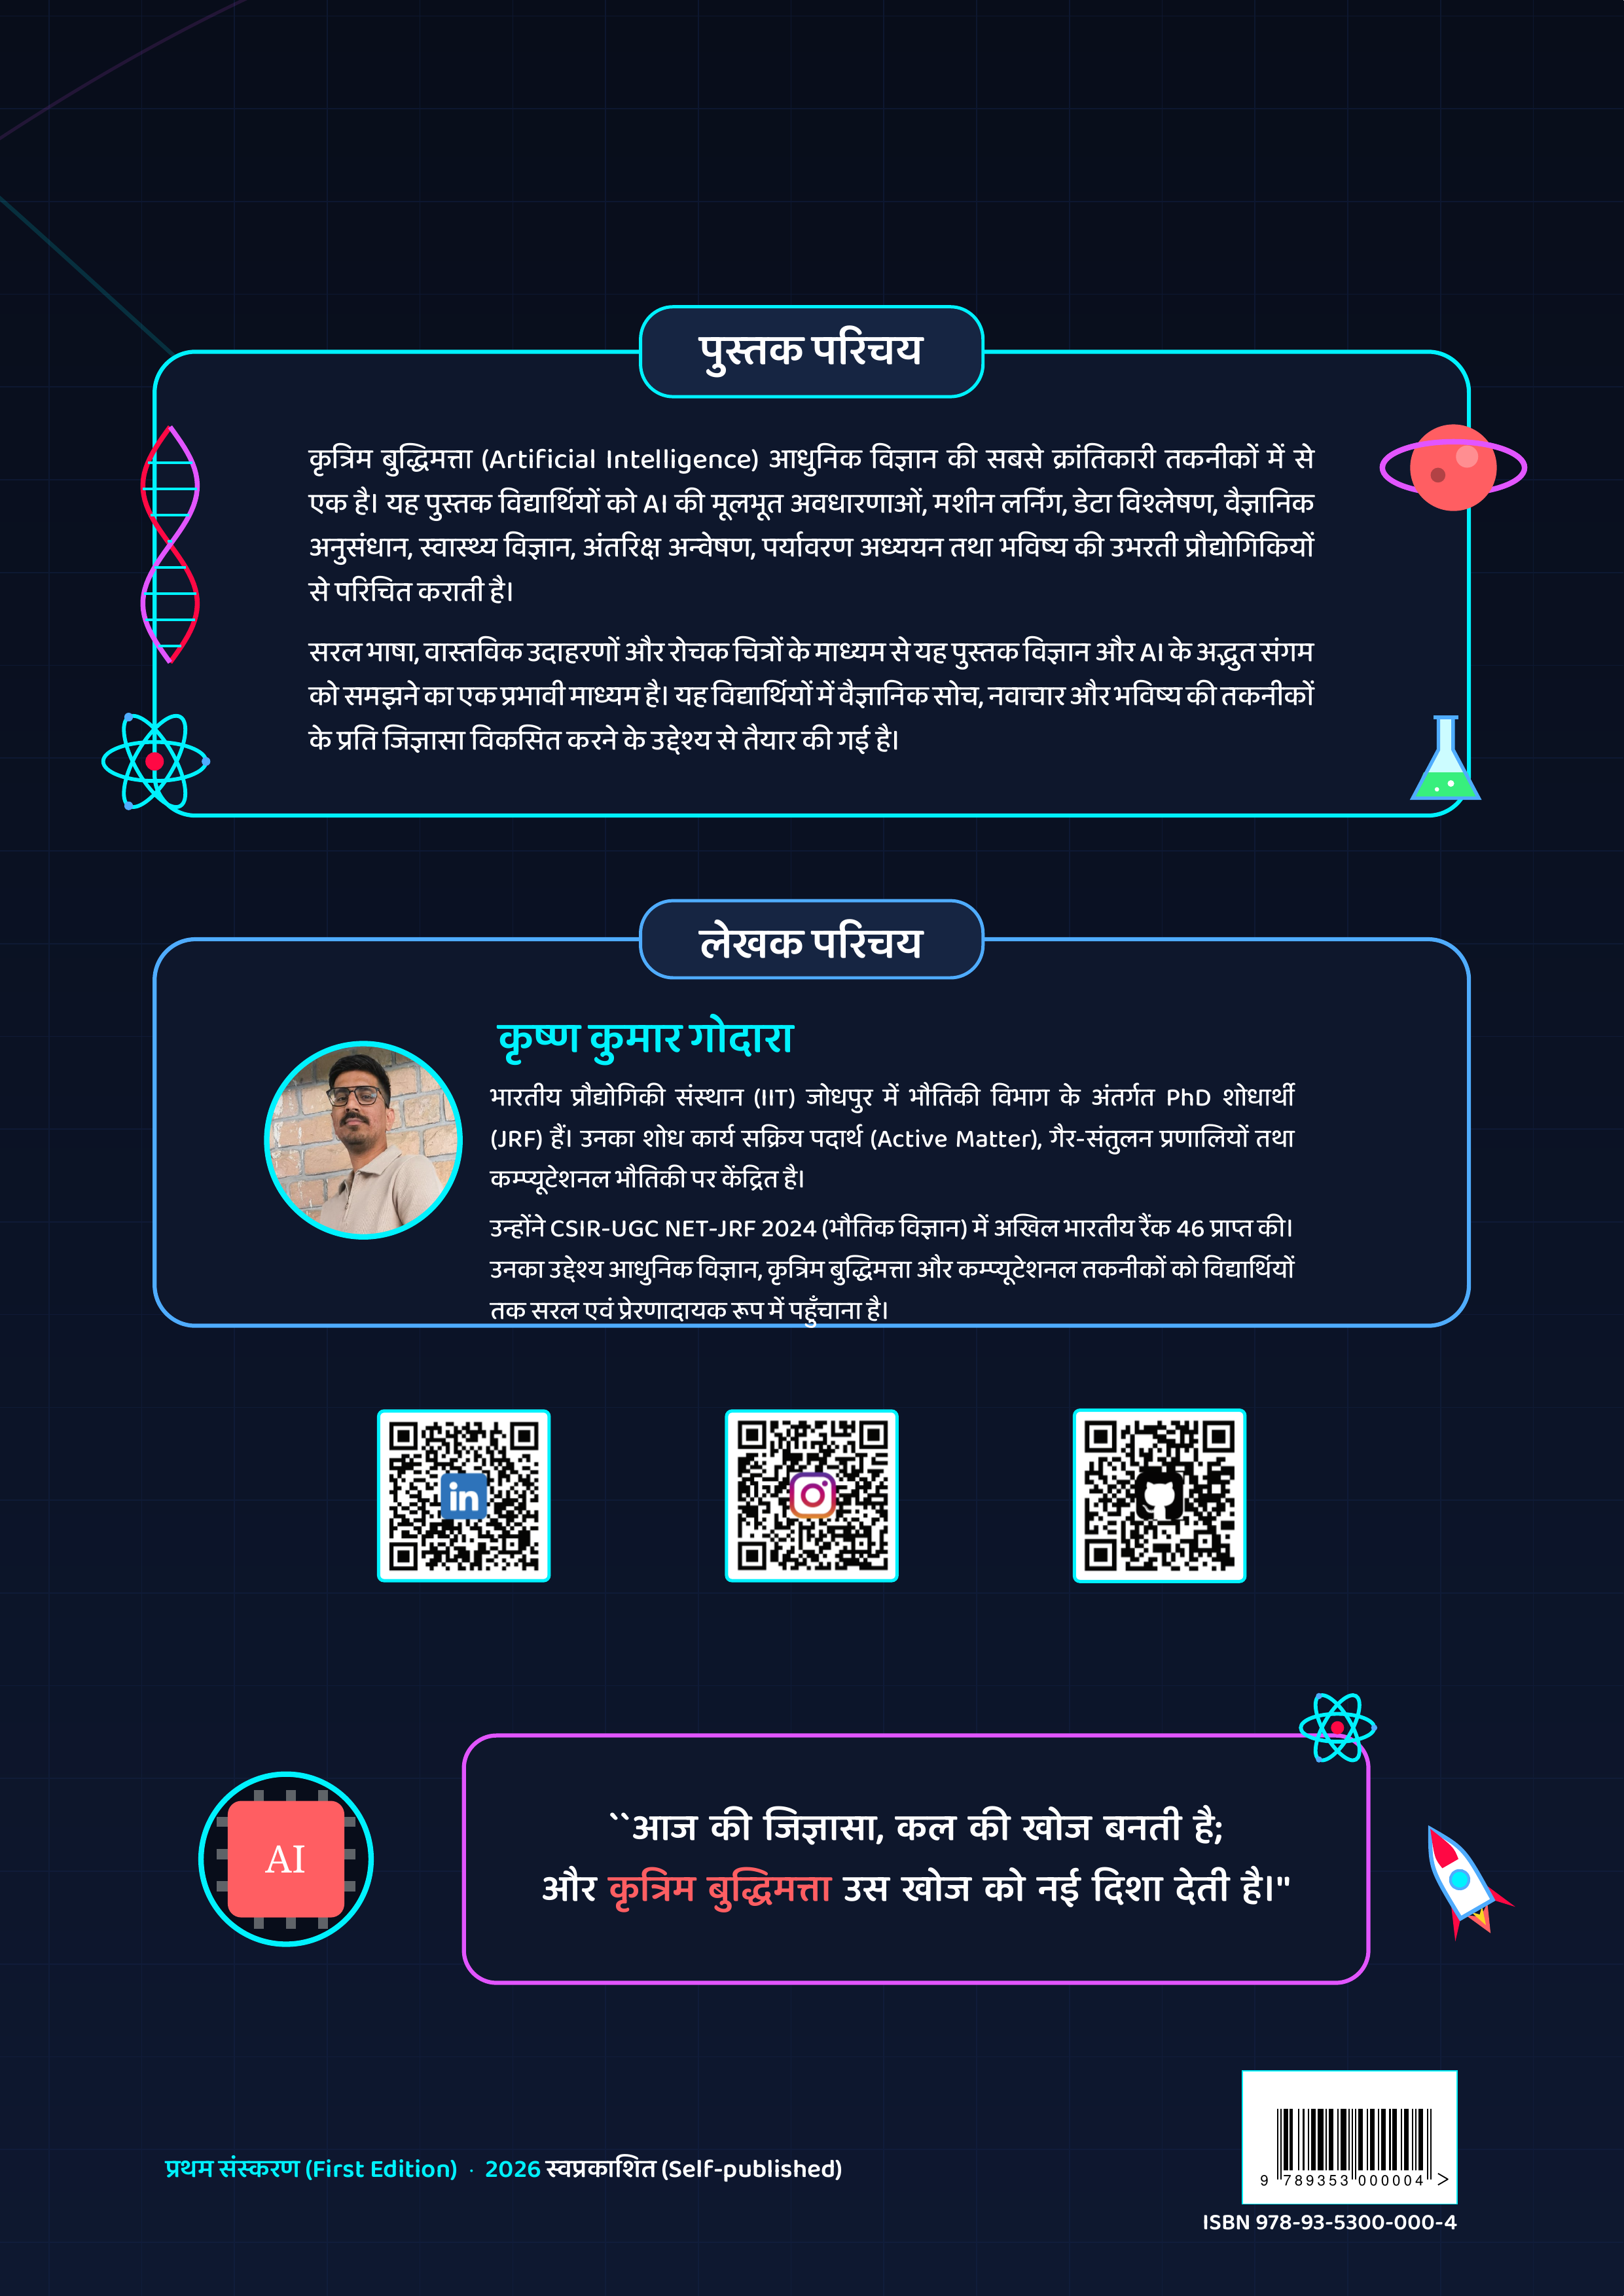
\includegraphics[width=\coverW cm,height=\coverH cm]{back-hi-69.png}};
  % --- front cover (right) ---
  \node[anchor=south west,inner sep=0] at ($(O)+(\bleed+\coverW+\spine,\bleed)$)
    {
\includegraphics[width=\coverW cm,height=\coverH cm]{front-hi-01.png}};
  % --- spine (centre) ---
  \fill[cvBgDark] ($(O)+(\bleed+\coverW,\bleed)$) rectangle ($(O)+(\bleed+\coverW+\spine,\bleed+\coverH)$);
  \node[rotate=90,text=white,font=\spinefont,scale=0.42]
    at ($(O)+(\bleed+\coverW+\spine/2, \bleed+\coverH/2)$)
    {विज्ञान में कृत्रिम बुद्धिमत्ता \quad\textbullet\quad K. K. Godara};
  % --- crop marks at the four trim corners ---
  \def\cm{0.55}
  \foreach \cx/\cy/\dx/\dy in {%
     \bleed/\bleed/-1/-1, {\bleed+2*\coverW+\spine}/\bleed/1/-1,
     \bleed/{\bleed+\coverH}/-1/1, {\bleed+2*\coverW+\spine}/{\bleed+\coverH}/1/1}{
     \draw[cvNeonCyan,line width=0.3pt]
        ($(O)+(\cx,\cy)$) -- ($(O)+(\cx+\dx*\cm,\cy)$);
     \draw[cvNeonCyan,line width=0.3pt]
        ($(O)+(\cx,\cy)$) -- ($(O)+(\cx,\cy+\dy*\cm)$);}
  % --- spine fold guide marks (top & bottom) ---
  \foreach \sx in {\bleed+\coverW, \bleed+\coverW+\spine}{
     \draw[cvNeonCyan,line width=0.3pt] ($(O)+(\sx,\bleed+\coverH)$) -- ($(O)+(\sx,\bleed+\coverH+\cm)$);
     \draw[cvNeonCyan,line width=0.3pt] ($(O)+(\sx,\bleed)$) -- ($(O)+(\sx,\bleed-\cm)$);}
\end{tikzpicture}
\end{document}
